\subsection{Trie index} \label{TRIEsubsec:trie}

To find an optimal alignment, we generally need to consider all reference graph
nodes $u \in \RG$ as possible starting nodes. Thus, optimal aligners
\pasgal~\cite{jain_accelerating_2019} and
\bitparallel~\cite{rautiainen_bitparallel_2019} brute-force through all
possible starting nodes $u \in \RG$.

To more efficiently handle arbitrary starting positions for alignments, we
extend the reference graph with a trie (referred to as \emph{suffix tree}
in~\cite{dox2018efficient}) to effectively align from all possible starting
nodes \emph{simultaneously}.

\paragraph{Single Starting State}
In the trie approach, abstraction nodes are added to the graph, each of which
corresponds to a set of nodes in $\RG$ that correspond to the same prefix. In
the following, we formalize this approach.

Concretely, we extend $\RG$ by a \emph{trie of depth $D$}, resulting in graph
$\TG=(\TGV,\TGE)$. Our goal is that all paths in $\RG$ that have length $D$ and
end in $v \in \RGV$ correspond to paths in $\TG$ starting from a single source
$\epsilon$ to $v \in \TGV$, where $\epsilon$ represents the empty string. This
correspondence ensures that it suffices to consider only paths in $\TG$ starting
from the source $\epsilon$. In particular, each alignment on $\TG$ can
be translated into an alignment on $\RG$ (we omit this translation
here).

%\begin{floatingfigure}[l]{0.46\textwidth}
\begin{figure}[H]
	\centering
	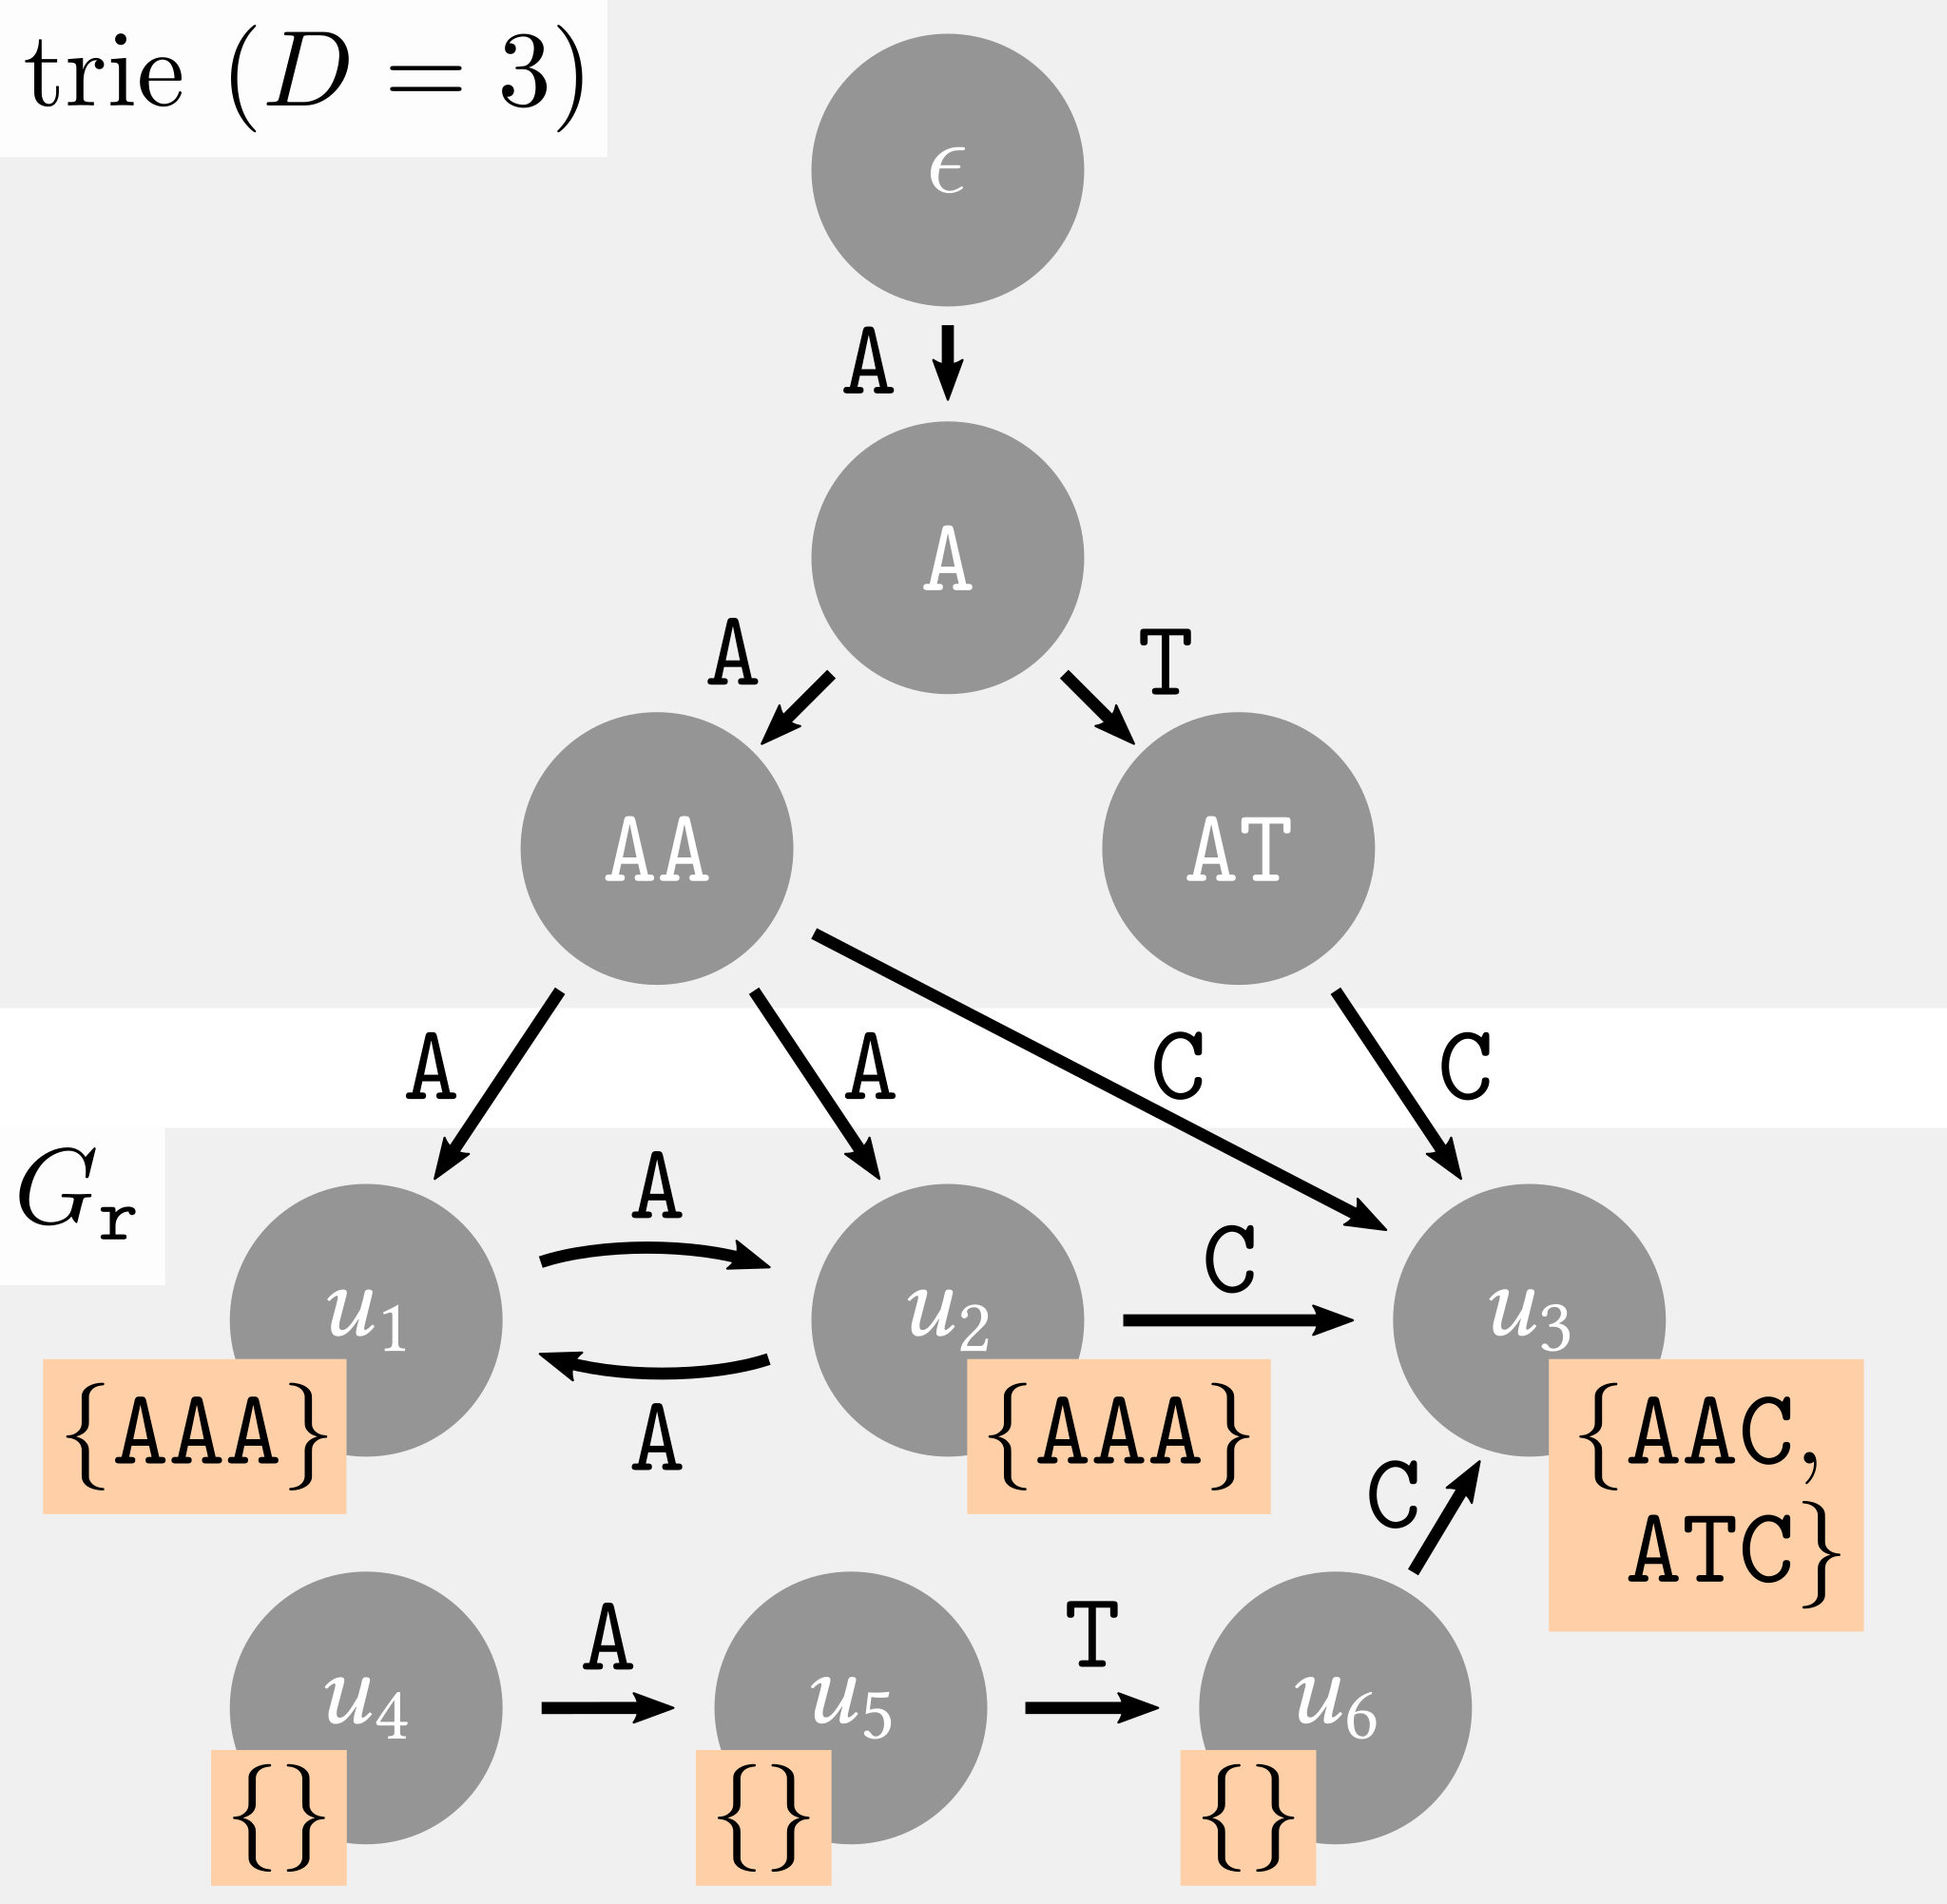
\includegraphics[width=0.43\linewidth]{\dir/figs/tree}
	\caption[Indexing the reference with a trie]{$\TG$ enables semi-global alignment by extending $\RG$ with a trie.}
	\label{TRIEfig:trie}
\end{figure}

\cref{TRIEfig:trie} shows an example trie. To construct it, we first associate with
every node $v \in \RGV$ the set $\mathcal{S}_v$ of its $D$-mers (orange boxes in
\cref{TRIEfig:trie}): spells of paths ending in $v$ and of length $D$. Our goal is
then to use paths in the trie to spell these $D$-mers.

Second, we construct the trie nodes from all prefixes of these $D$-mers:
%
$$ \TGV:= \RGV \cup
\bigcup_{v \in \RGV} \left\{s[0:i] \,\middle|\, \begin{array}{{@{}c@{}}}
	s \in \mathcal{S}_v, \\
	0 \leq i < D
\end{array} \right\}.
$$

Third, we add edges within the trie, which ensure that paths from $\epsilon$ to
any trie node $s$ spell $s$. Formally, whenever $s \concat \ell \in \TGV$, we add
an edge $(s,s \concat \ell, \ell)$ to $\TGE$, where ``$\concat$'' denotes string
concatenation.
%
Finally, we add edges between the trie and the reference graph, which ensure
that any $D$-mer of any node $v \in \RGV$ can be spelled by a walk from
$\epsilon$ to $v$. Formally, if $s \concat \ell \in \mathcal{S}_v$, then
$(s,v,\ell) \in \TGE$.

Importantly, extending $\RG$ to $\TG$ is compatible with the construction of the alignment graph and all other
optimizations. In particular, when searching for a shortest path in the
alignment graph constructed from $\TG$, it suffices to only consider starting
node $\langle \epsilon, 0 \rangle$.

\paragraph{Reducing Size of Trie} \label{TRIEpara:reducing_trie}
We can reduce the size of the trie by removing specific trie nodes.
%
In particular, we iteratively remove each trie leaf node $s \cdot \ell \in \TGV$ with a unique outgoing edge $(s \cdot \ell, v, \ell')$ to a reference graph node $v \in \RGV$.
%
To compensate for removing node $s \cdot \ell$, we introduce a new edge $(s, u, \ell)$ to a node $u \in \RGV$ with an edge $(u,v,\ell')$ (such a node must exist according to the construction of $\TG$).
%
For example, in \cref{TRIEfig:trie}, we (i)~remove node \texttt{AT} including its edges $(\texttt{A},\texttt{AT},\texttt{T})$ and $(\texttt{AT},u_3,\texttt{C})$, but (ii)~introduce an edge $(\texttt{A},u_2,T)$.

This optimization is lossless, as the $D$-mer $s \cdot \ell \cdot \ell' \in \mathcal{S}_v$ can still be spelled by the path from $\epsilon$ to $s$, extended by $(s, u, \ell)$ and $(u, v, \ell')$.